\documentclass[12pt,a4paper]{article}
\usepackage[T1]{fontenc}
\usepackage[polish]{babel}
\usepackage[utf8]{inputenc}
\usepackage{lmodern}
\usepackage{amsmath}
\usepackage{hyperref}
\usepackage{array}
\usepackage{pdflscape}
\usepackage{amsfonts}
\usepackage{graphicx}
\usepackage{longtable}
\usepackage{float}
\selectlanguage{polish}
\usepackage{url}


\usepackage[top=2cm, bottom=2cm, left=3cm, right=3cm]{geometry}
\makeatletter
\newcommand{\linia}{\rule{\linewidth}{0.4mm}}

\newcommand{\Ameryk}{${}^{241}_{}{}$Am }

\renewcommand{\maketitle}{\begin{titlepage}
    \vspace*{1cm}
    \begin{center}\small
    Uniwersytet Warszawski\\
    Wydział Fizyki\\
   Raport z Indywidualnej pracay w laboratorium badawczym
    \end{center}
    
\begin{figure}[h]
    \centering
    
\includegraphics[scale=0.5]{logo.jpg}
    \end{figure}


    \vspace{3cm}
    \noindent\linia
    \begin{center}
      \LARGE \textsc{\@title}
         \end{center}
     \linia
    \vspace{0.5cm}
    \begin{flushright}
    \begin{minipage}{5cm}
    \textit{\small Autor:}\\
    \normalsize \textsc{\@author} \par
    \end{minipage}
    \vspace{5cm}
    
     \end{flushright}
    \vspace*{\stretch{6}}
    \begin{center}
    \@date
    \end{center}
         \end{titlepage}}
    
\makeatother
\author{Filip Kowalski }
\title{Pomiar grubości foli mylarowych przy pomocy promieniowania $\alpha$} 

%pzc
\begin{document}
\maketitle
\begin{abstract}
W czasie ćwiczenia próbowano oszacować grubość foli mylarowych przy pomocy promieniowania $\alpha$. 
\end{abstract}
\section{Wstęp}
Podczas ćwiczenia przygotowano próbki pomiarowe, następnie dokonano kalibracji układu przy pomocy pulsera i źródełka proieniowania $\alpha$. Następnie zmierzono energie cząstek $\alpha$ po przejściu przez próbki mylarowe. Korzystając z danych pomiarowych oraz wyników wygenerowanych przy pomocy programu SRIM, obliczono grubości folii.

\subsection{Kalibracja}
W celu kalibracji układu wykorzystano promieniowanie źródła \Ameryk oraz sygnał generowany przez pulser. Przy wykorzystaniu detektora krzemowego, mierzono kanał promieniowania $\alpha$. Podczas wszystkich pomiarów do detektora przyłożone było napięcie 55 V. Aby móc powiązać kanał z odpowiadającą mu energią cząstki $\alpha$, do kalibracji wykorzystano sygnał z puslera. Zmieniając napięcie  na pulserze, zmierzono zależność kanału od przyłożonego napięcia. Wykres przedstawiający zmierzone wartości przedstawiono na rysunku \ref{kalibracja}. Znając napięcie na pulserze odpowiadające danemu pikowi oraz numer kanału środka piku (dane umieszczone w tabeli \ref{kalibracja_tab}), oraz energię $\alpha$ emitowaną przez \Ameryk  (5.486 MeV) dopasowano funkcję pozwalającą obliczyć energię cząstki padającej na detektor znając jej numer kanału. Dopasowana funkcja, wraz z parametrami dopasowania znajduje się na wykresie \ref{dopasowanie_prostej}. Zdecydowano się na dopasowanie wielomianu drugiego stopnia, ponieważ daje dokładniejsze przewidywania (przy dopasowaniu funkcji liniowej dopasowana krzywa cyklicznie przewidywała zbyt małe i zbyt duże wartości co stwarzało podstawy do dodania kolejnego stopnia swobody). 

\begin{table}[]
\centering
\caption{My caption}
\label{kalibracja_tab}
\begin{tabular}{|c|c|ccl}
\cline{1-4}
\multicolumn{2}{|c|}{Pomiar w wykonany w dniu 2017.11.30} & \multicolumn{2}{c|}{Pomiar wykonany w dniu 2017.12.07}                                &  \\ \cline{1-4}
Numer kanału        & Napięcie na pulserze {[}V{]}        & \multicolumn{1}{c|}{Numer kanału} & \multicolumn{1}{c|}{Napięcie na pulserze {[}V{]}} &  \\ \cline{1-4}
553,35187           & 0,03                                & \multicolumn{1}{c|}{851,37852}    & \multicolumn{1}{c|}{0,05}                         &  \\ \cline{1-4}
851,57069           & 0,05                                & \multicolumn{1}{c|}{1147,46812}   & \multicolumn{1}{c|}{0,07}                         &  \\ \cline{1-4}
1147,68439          & 0,07                                & \multicolumn{1}{c|}{1443,65577}   & \multicolumn{1}{c|}{0,09}                         &  \\ \cline{1-4}
1443,94784          & 0,09                                & \multicolumn{1}{c|}{1742,11607}   & \multicolumn{1}{c|}{0,11}                         &  \\ \cline{1-4}
1742,44734          & 0,11                                & \multicolumn{1}{c|}{2038,30311}   & \multicolumn{1}{c|}{0,13}                         &  \\ \cline{1-4}
2038,90259          & 0,13                                & \multicolumn{1}{c|}{2336,88623}   & \multicolumn{1}{c|}{0,15}                         &  \\ \cline{1-4}
2337,63571          & 0,15                                & \multicolumn{1}{c|}{2932,71001}   & \multicolumn{1}{c|}{0,19}                         &  \\ \cline{1-4}
2932,98088          & 0,19                                & \multicolumn{1}{c|}{3228,62791}   & \multicolumn{1}{c|}{0,21}                         &  \\ \cline{1-4}
3229,44276          & 0,21                                &                                   &                                                   &  \\ \cline{1-2}
\end{tabular}
\end{table}



\begin{figure}[H]
\centering
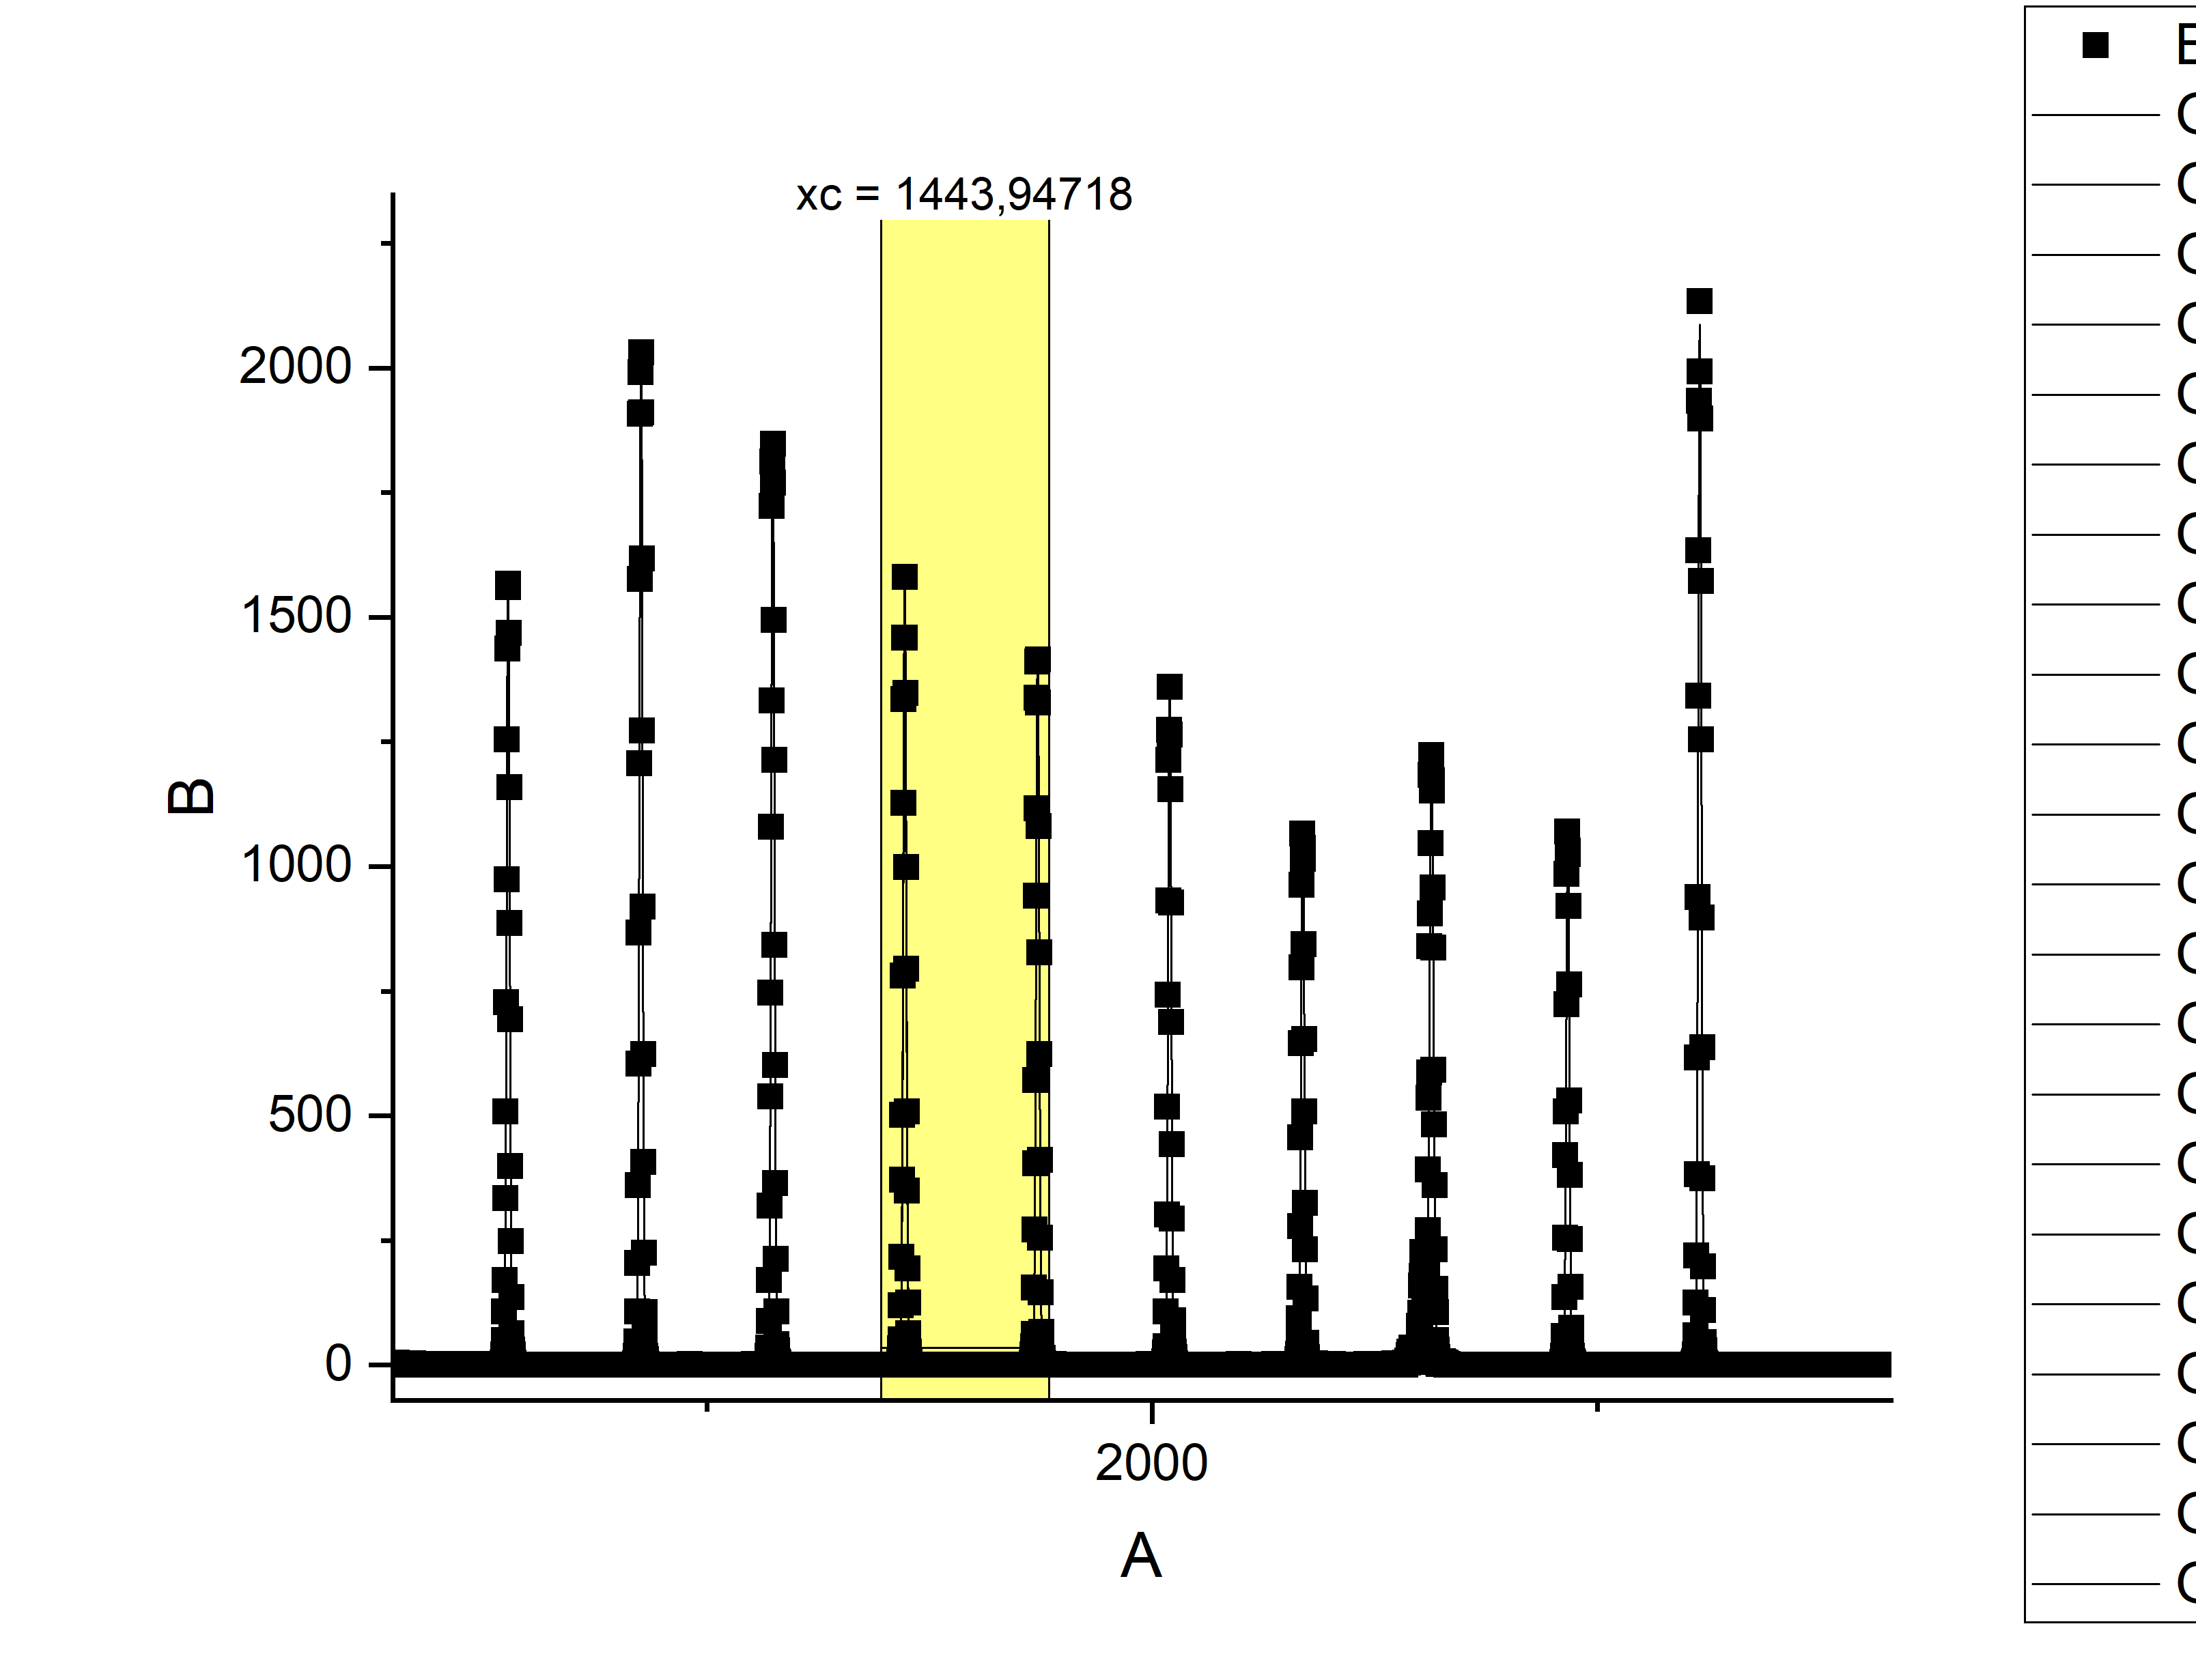
\includegraphics[scale=0.5]{kalibracja.png}
\caption{Zliczenia w zależności od kanału - pomiar kalibracyjny}
\label{kalibracja}
\end{figure}

\begin{figure}[H]
\centering
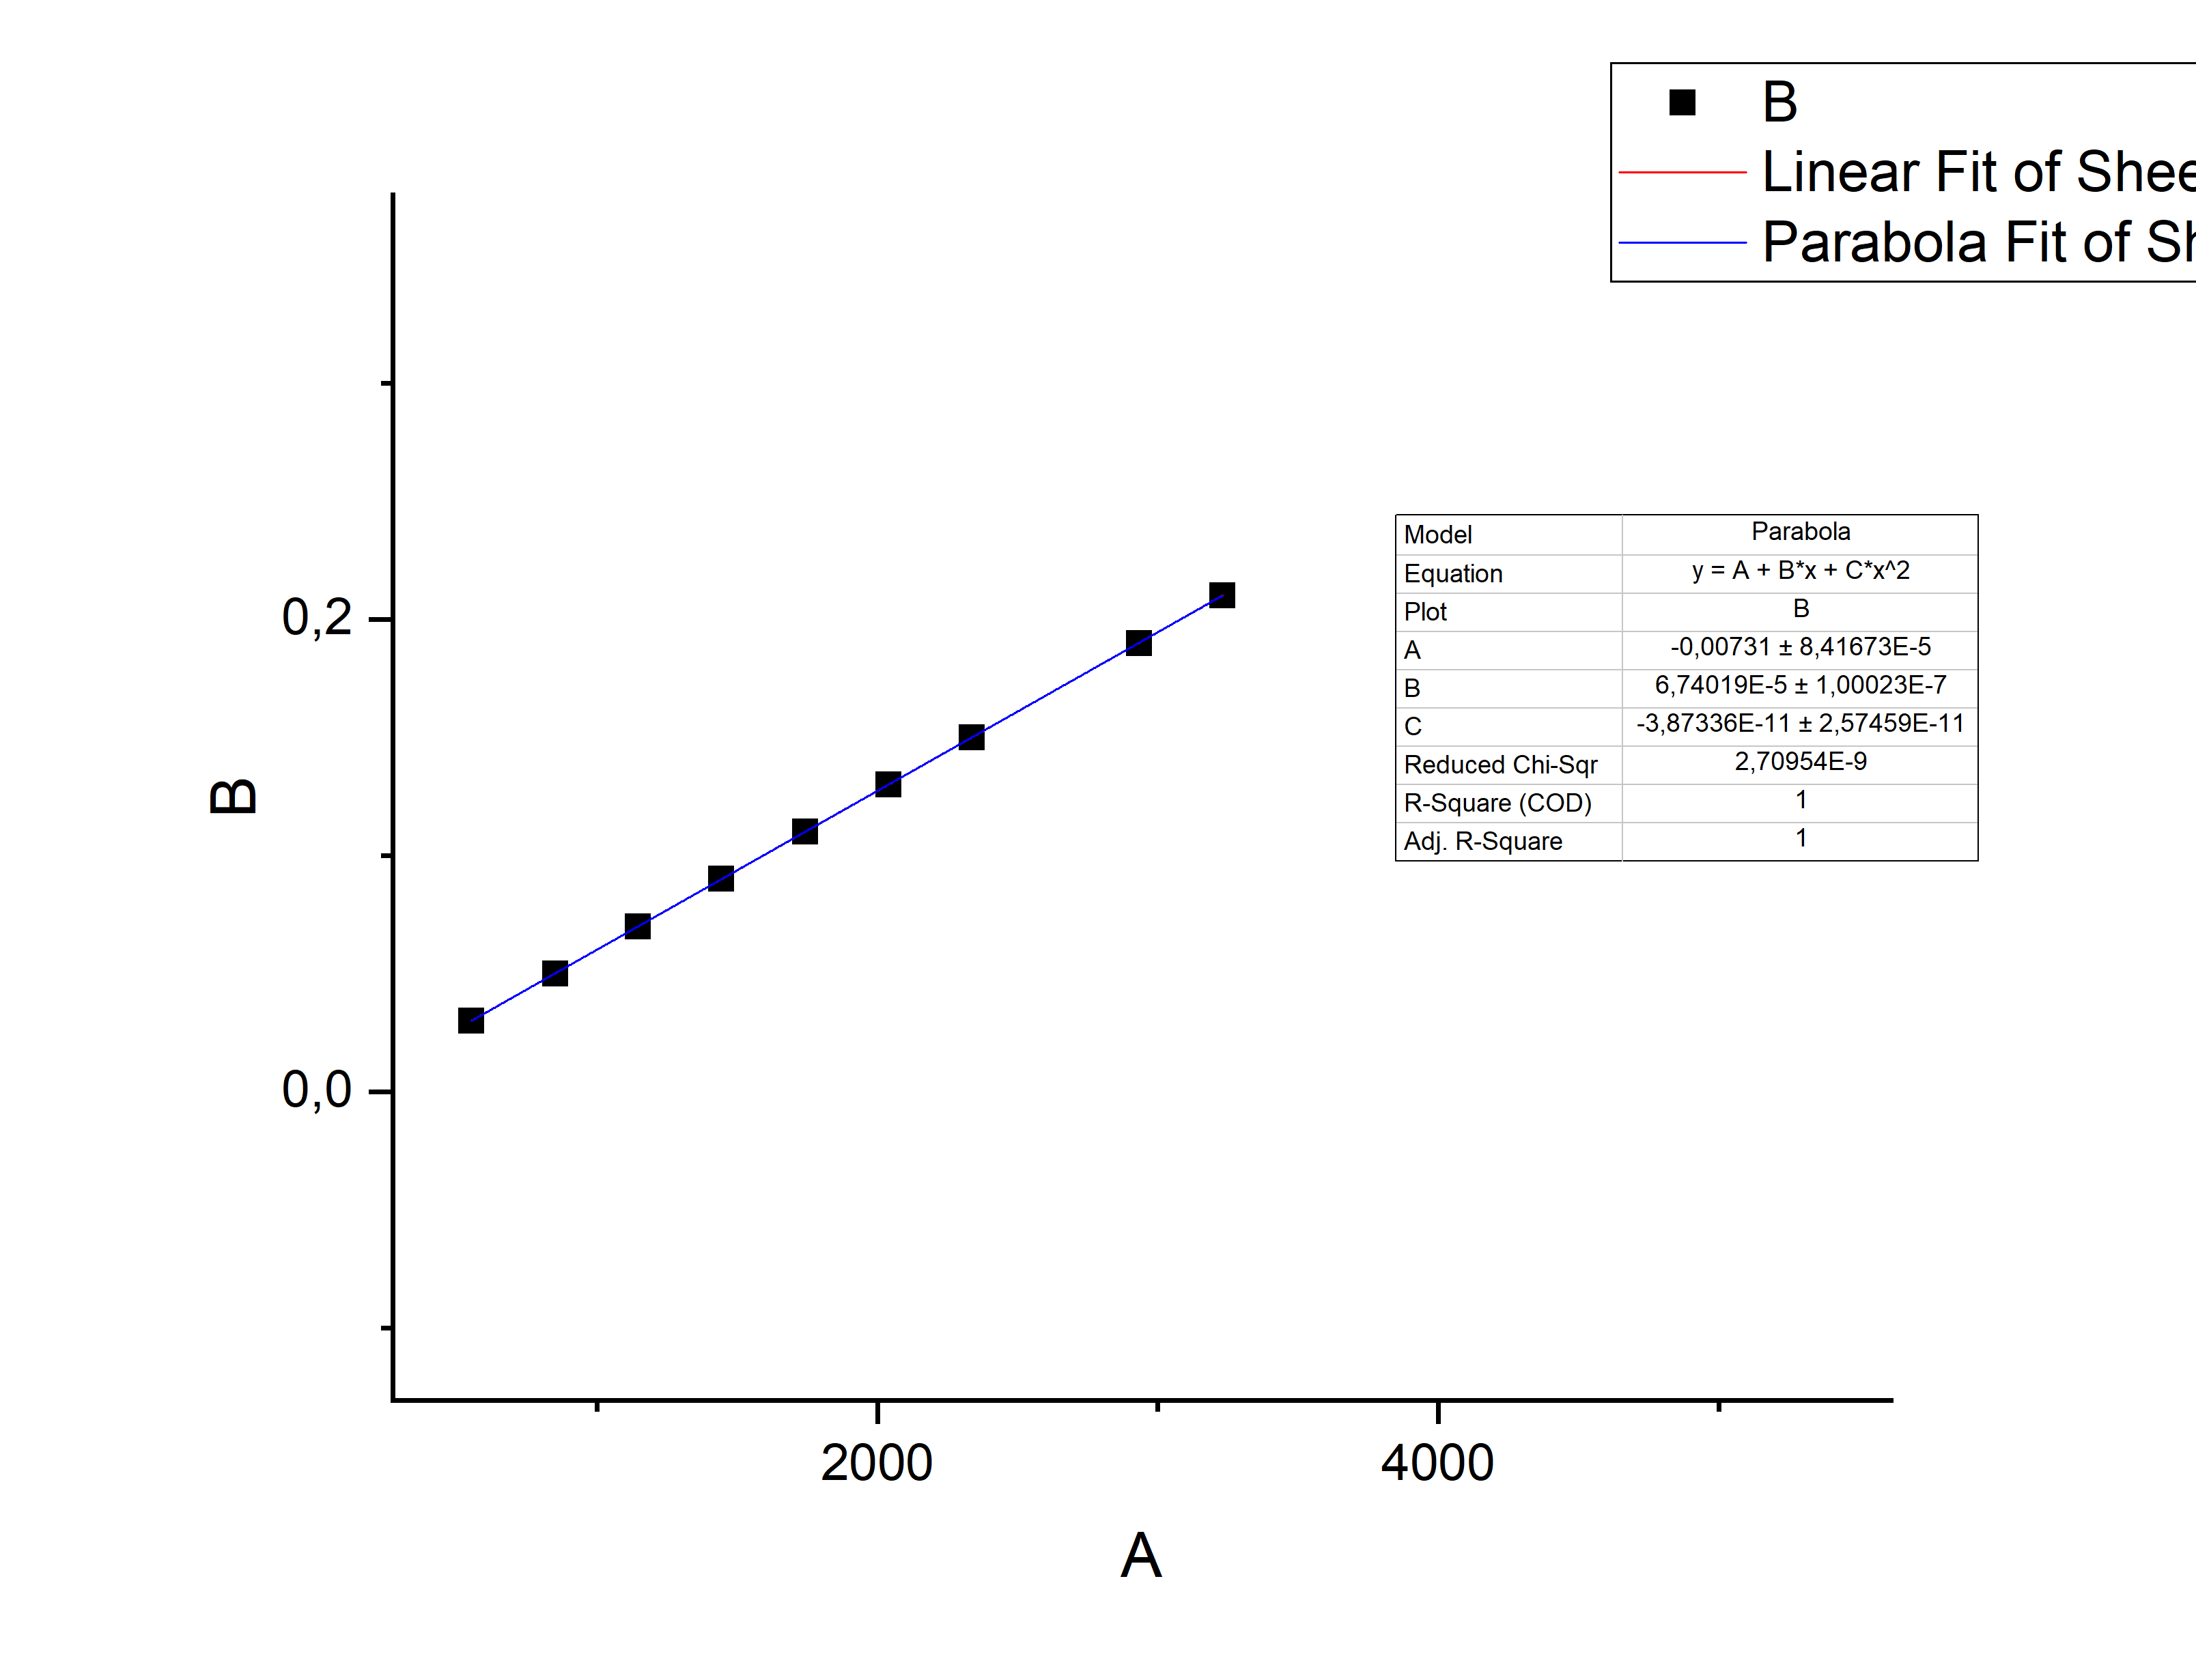
\includegraphics[scale=0.5]{dopasowanie.png}
\caption{Zliczenia w zależności od kanału - pomiar kalibracyjny}
\label{dopasowanie_prostej}
\end{figure}





\subsection{Pomiar}

W celu zmierzenia grubości folii mylarowych, najpierw przygotowano próbki nalepiając kawałki folii na metalowe okienka. Najlepiej sprawdzająca się technika (szczególnie dla cienkich folii, mających tendencję do zwijania się) polegała na przyłożeniu metalowego okienka do arkuszu folii znajdującej się pomiędzy dwoma kartkami papieru a następnie przy pomocy skalpela odcięciu, po zewnętrznym obrysie okienka, potrzebnej ilości folii. Następnie odcięty kawałek należało przykleić do okienka. Tak przygotowane próbki umieszczano w komorze próżniowej i mierzono kanał padania cząstki $\alpha$ przechodzącej przez próbkę. Wyniki przykładowego pomiaru zamieszczono na rysunku  \ref{przykladowy_pomiar}.




\begin{figure}[H]
\centering
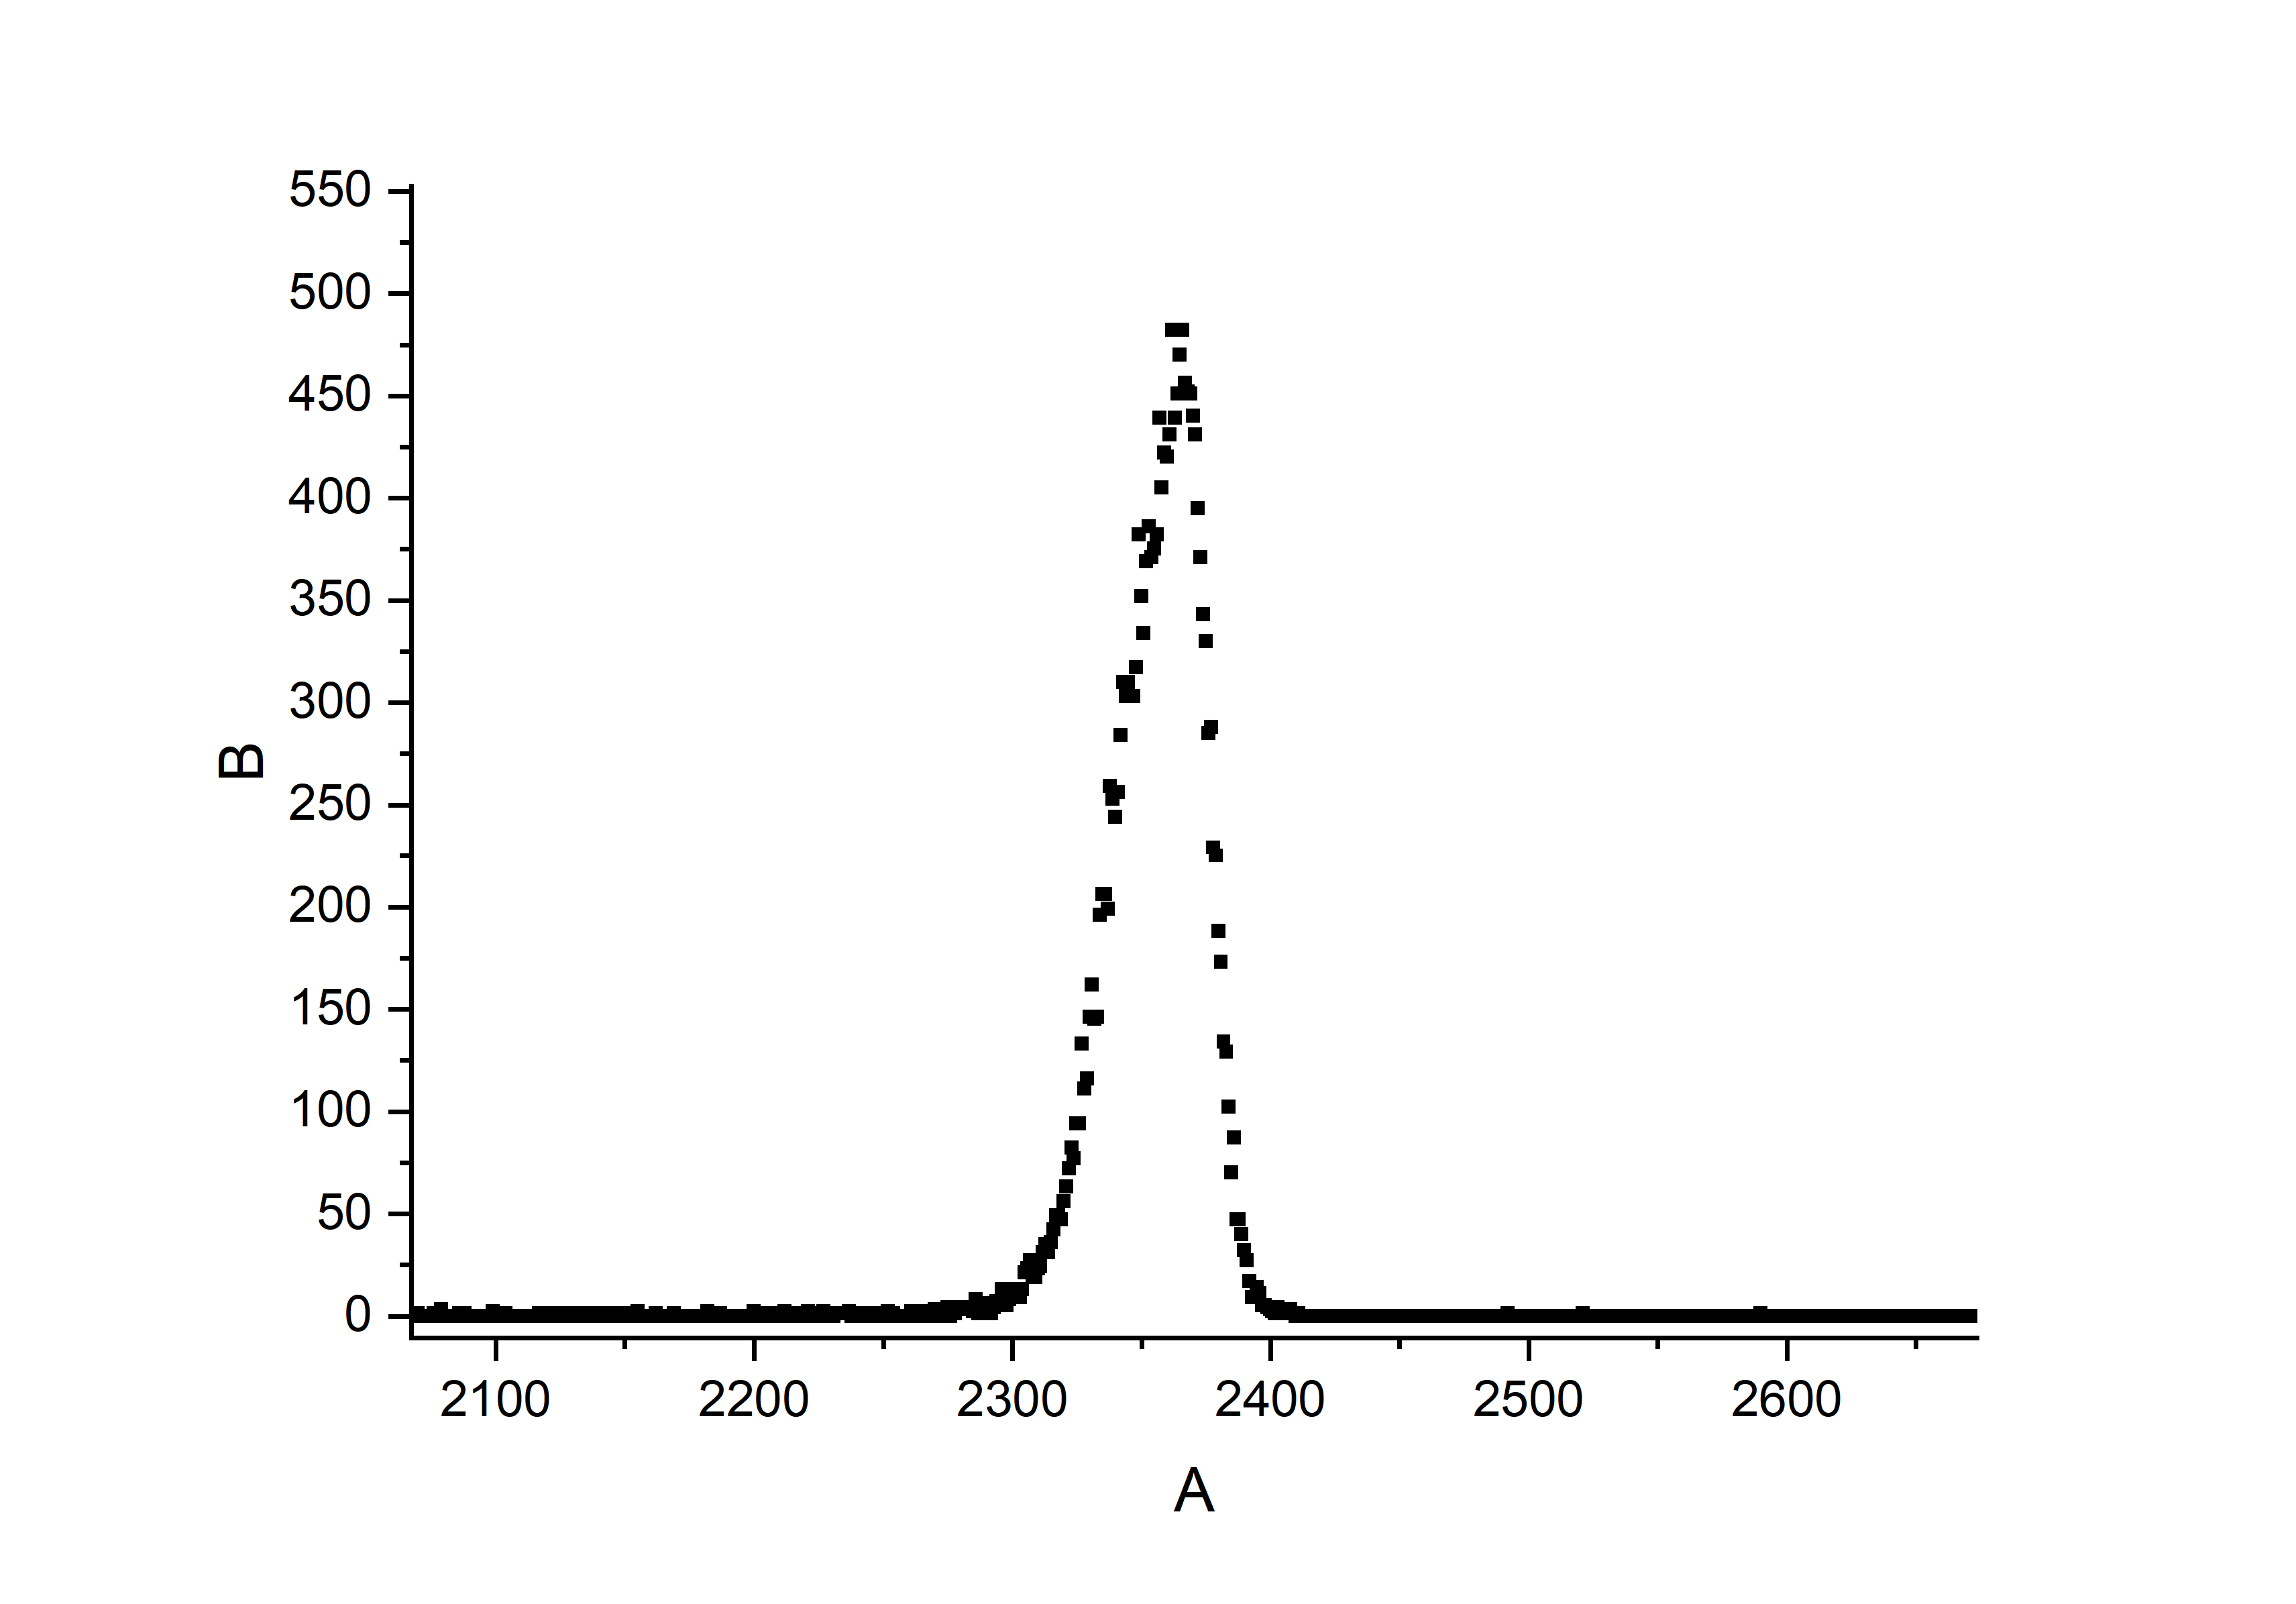
\includegraphics[scale=0.5]{Enlarged.png}
\caption{Wykres zliczeń w zależności od kanału dla próbki E. Pomiar z dnia 17.11.30}
\label{przykladowy_pomiar}
\end{figure}


\subsection{Analiza danych}
Dla każdej próbki do zmierzonej zależności ilości zliczeń od kanału dopasowano krzywą Gaussa w celu określenia położenia maksimum piku. Kożystając z wyznaczonych podczas kalibracji parametrów można było przeliczyć numer kanału na energię cząstki $\alpha$ po przejściu przez daną próbkę. 
Do wygenerowania danych potrzebnych do zamiany energii na grubość próbki skorzystano z programu SRIM. W programie wygenerowano zależność energii cząstki $\alpha$ do zasięgu jaki powinna osiągnąć poruszając się w ośrodku złożonym z mylaru. jh,


\section{Prezentacja wyników}













\section{Dyskusja wyników i obserwacja}
Dyskusja 

\begin{thebibliography}{9}
\bibitem{ins} 
Instrukcja do ćwiczenia
\url{http://psi.fuw.edu.pl/bin/view/IPWb/PojemnoscCieplnaZarowki}
\end{thebibliography}
\end{document}